% mycsrf 'for beeing included' snippet template
%
% (c) Karsten Reincke, Frankfurt a.M. 2012, ff.
%
% This text is licensed under the Creative Commons Attribution 3.0 Germany
% License (http://creativecommons.org/licenses/by/3.0/de/): Feel free to share
% (to copy, distribute and transmit) or to remix (to adapt) it, if you respect
% how you must attribute the work in the manner specified by the author(s):
% \newline
% In an internet based reuse please link the reused parts to mycsrf.fodina.de
% and mention the original author Karsten Reincke in a suitable manner. In a
% paper-like reuse please insert a short hint to mycsrf.fodina.de and to the
% original author, Karsten Reincke, into your preface. For normal quotations
% please use the scientific standard to cite
%

\section{Prozessgüte und Prozessreife einzelner Ketten}

Wir werden in den folgenden Abschnitten die Ergebnisse unserer Tests nur
summarisch protokollieren. Trotzdem ist die Reproduzierbarkeit und
Überprüfbarkeit auf folgende Weise gewährleistet:

\begin{itemize}
  \item In den Quellen zu diesem Text\footcite[vgl.][\nopage wp]{Reincke2019a}
  findet sich auch der Ordner \texttt{chain-evaluation}. Sofern nicht von unser
  Distribution generell bereitgestellt, enthält dieser Ordner alle
  IO-(Zwischen)-Ergebnisse und alle Tools resp. Makefiles, die auf den
  definierten Wegen benötigt resp. erzeugt werden.
  \item Als erstes haben wir in jedem Frontend -- sei es per Import\footnote{die
  entsprechende XML Datei ist beigelegt}, sei es manuell -- in etwa folgende
  Eingabe zu erzeugen versucht:
  \begin{center}
    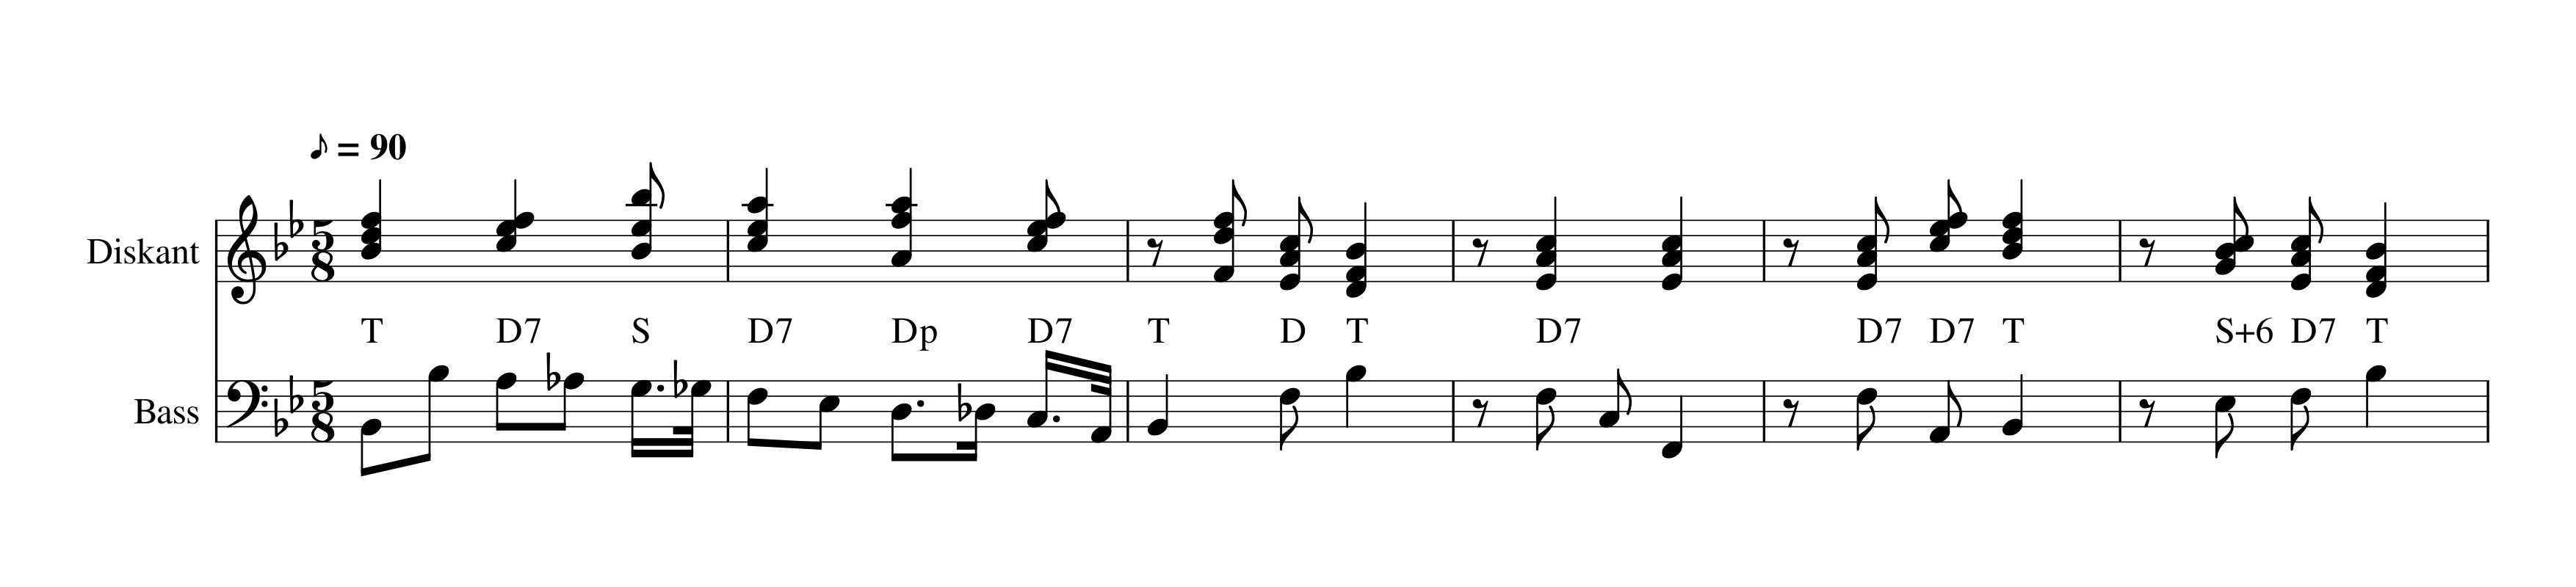
\includegraphics[width=0.9\textwidth]{frontends/musescore/cadenca3-musescore-300dpi.png}
  \end{center}
  Wir wissen ja bereits, dass die ausgefeilte Harmoniedokumentation in keinem
  Frontend möglich ist. Wir erwarten technisch aber, dass die vereinfachte
  Darstellung problemlos ins Backend übertragen wird und -- bei MusiX\TeX\ und
  LilyPond -- manuell durch die besseren Versionen ersetzbar ist, also
  bei MusiX\TeX\ durch \acc{harmony}-Konstrukte und bei LilyPond durch die unser
  kleinen Zusatzbibliothek.
  \item Danach haben wir in jedem Fronted alle möglichen Exporte angestoßen und
  die Ergebnisse in einem Ordner \texttt{from-frontend-to} abgelegt.
  \item Für jeden Weg, der vom Fontend aus gegangen werden kann, gibt es im
  Frontendordner einen Ordner mit der entsprechenden Nummer.
  \item Wird der Output des Frontends gemäß der Wegdefinition direkt als Input für
  das Backend verwendet, findet sich im Wegordner ein entsprechendes \LaTeX- und
  Makefile und die so generierte PDF-Datei.
  \item Wird der Output des Frontends dagegen einem Konverter vorlegt, enthält
  der Wegeordner auch den Output des Konverters. \LaTeX- und Makefile
  operieren dann auf und mit diesen Daten.
  \item Dort, wo das entsprechende Frontend oder der Konverter nicht von unserer
  Referenzdistribution\footnote{Ubuntu 18.04} bereitgestellt wird, haben wir die
  entsprechenden Pakete beigelegt.
\end{itemize}

Mit diesen Materialien haben wir die folgenden Ergebnisse erzeugt.

\subsection{W01: Easy\-ABC \ra\ \LaTeX+ABC (0.8/0.56)}

Die aus Easy\-ABC als \acc{abc}-Code exportierte Referenzkadenz III kann
technisch direkt in das \LaTeX-Backend eingefügt werden. Das Ergebnis ist
graphisch perfekt. Allerdings wird die vorgegebene Tempoangabe \texttt{\Acht=90}
während des Exports/Imports in \texttt{\Vier=45} umgewandelt. Das ist bei einem
\texttt{5/8}-Takt nicht sinnvoll und muss manuell korrigiert werden. Damit
ergibt sich eine Prozessgüte von \texttt{0.8} und eine normierte Prozessreife von
\texttt{((4+3-0)*0.8)/10=0.56}.

\subsection{W02: Easy\-ABC \ra\ xml2abc \ra\ \LaTeX+ABC: (1.0)}

2

\subsection{W03: Easy\-ABC \ra mxml2abc \ra\ \LaTeX+ABC: (1.0)}

3

\subsection{W04: Easy\-ABC \ra\ abc2ly \ra\ ly2abc \ra\ \LaTeX+ABC: (1.0)}

4

\subsection{W05: Easy\-ABC \ra mxml2ly \ra\ ly2abc \ra\ \LaTeX+ABC: (1.0)}

5

\subsection{W06: Easy\-ABC \ra xml2ly \ra\ ly2abc \ra\ \LaTeX+ABC: (1.0)}

6

\subsection{W07: Rose\-garden \ra\ xml2abc \ra\ \LaTeX+ABC: (1.0)} 

7

\subsection{W08: Rose\-garden \ra\ mxml2abc \ra\ \LaTeX+ABC: (1.0)} 

8

\subsection{W09: Rose\-garden \ra\ mxml2ly \ra\ ly2abc \ra\ \LaTeX+ABC: (1.0/1.0)} 

9

\subsection{W10: Rose\-garden \ra\ xml2ly \ra\ ly2abc \ra\ \LaTeX+ABC: (1.0)} 

10

\subsection{W11: Muse\-Score \ra\ xml2abc \ra\ \LaTeX+ABC: (1.0)} 

11

\subsection{W12: Muse\-Score \ra\ mxml2abc \ra\ \LaTeX+ABC: (1.0)}

12

\subsection{W13: Muse\-Score \ra\ mxml2ly \ra\ ly2abc \ra\ \LaTeX+ABC: (1.0)} 

13

\subsection{W14: Muse\-Score \ra\ xml2ly \ra\ ly2abc \ra\ \LaTeX+ABC: (1.0)}

14

\subsection{W15: Denemo \ra\ xml2abc \ra\ \LaTeX+ABC: (1.0)}

15

\subsection{W16: Denemo \ra\ mxml2abc \ra\ \LaTeX+ABC: (1.0)} 

16

\subsection{W17: Denemo \ra\ mxml2ly \ra\ ly2abc \ra\ \LaTeX+ABC: (1.0)} 

17

\subsection{W18: Denemo \ra\ xml2ly \ra\ ly2abc \ra\ \LaTeX+ABC: (1.0)} 

18

\subsection{W19: Canorus \ra\ xml2abc \ra\ \LaTeX+ABC: (1.0)} 

19

\subsection{W20: Canorus \ra\ mxml2abc \ra\ \LaTeX+ABC: (1.0)} 

20

\subsection{W21: Canorus \ra\ mxml2ly \ra\ ly2abc \ra\ \LaTeX+ABC: (1.0)} 

21

\subsection{W22: Canorus \ra\ xml2ly \ra\ ly2abc \ra\ \LaTeX+ABC: (1.0)} 

22

\subsection{W23: Texteditor \ra\ \LaTeX+ABC: (1.0)}

23

\subsection{W24: EasyABC \ra\ abc2mtex \ra\ \LaTeX+Musix\TeX: (1.0)} 

24

\subsection{W25: EasyABC \ra\ mxml2pmx \ra\ pmxab \ra\ \LaTeX+Musix\TeX: (1.0)} 

25

\subsection{W26: Rosegarden \ra\ mxml2pmx \ra\ pmxab \ra\ \LaTeX+Musix\TeX: (1.0)}

26

\subsection{W27: MuseScore \ra\ mxml2pmx \ra\ pmxab \ra\ \LaTeX+Musix\TeX: (1.0)}

27

\subsection{W28: Denemo \ra\ mxml2pmx \ra\ pmxab \ra\ \LaTeX+Musix\TeX: (1.0)} 

28

\subsection{W29: Canorus \ra\ mxml2pmx \ra\ pmxab \ra\ \LaTeX+Musix\TeX: (1.0)} 

29

\subsection{W30: Texteditor \ra\ \LaTeX+Musix\TeX: (1.0)}

30

\subsection{W31: Texteditor \ra\ pmxab \ra\ \LaTeX+Musix\TeX: (1.0)}

31

\subsection{W32: Easy\-ABC \ra xml2ly \ra\ Elysium \ra\ \LaTeX+LilyPond: (1.0)} 

32

\subsection{W33: Easy\-ABC \ra mxml2ly \ra\ Elysium \ra\ \LaTeX+LilyPond: (1.0)} 

33

\subsection{W34: Easy\-ABC \ra xml2ly \ra\ Frescobaldi \ra\ \LaTeX+LilyPond: (1.0)}

34

\subsection{W35: Easy\-ABC \ra mxml2ly \ra\ Frescobaldi \ra\ \LaTeX+LilyPond: (1.0)} 

35

\subsection{W36: Rosegarden \ra xml2ly \ra\ Elysium \ra\ \LaTeX+LilyPond: (1.0)}

36

\subsection{W37: Rosegarden \ra mxml2ly \ra\ Elysium \ra\ \LaTeX+LilyPond: (1.0)}

37

\subsection{W38: Rosegarden \ra xml2ly \ra\ Frescobaldi \ra\ \LaTeX+LilyPond: (1.0)}

38

\subsection{W39: Rosegarden \ra mxml2ly \ra\ Frescobaldi \ra\ \LaTeX+LilyPond: (1.0)}

39

\subsection{W40: MuseScore \ra xml2ly \ra\ Elysium \ra\ \LaTeX+LilyPond: (1.0)}

40

\subsection{W41: MuseScore \ra mxml2ly \ra\ Elysium \ra\ \LaTeX+LilyPond: (1.0)}

41

\subsection{W42: MuseScore \ra xml2ly \ra\ Frescobaldi \ra\ \LaTeX+LilyPond: (1.0)} 

42

\subsection{W43: MuseScore \ra mxml2ly \ra\ Frescobaldi \ra\ \LaTeX+LilyPond: (1.0)} 

43

\subsection{W44: Denemo \ra xml2ly \ra\ Elysium \ra\ \LaTeX+LilyPond: (1.0)} 

44

\subsection{W45: Denemo \ra mxml2ly \ra\ Elysium \ra\ \LaTeX+LilyPond: (1.0)} 

45

\subsection{W46: Denemo \ra xml2ly \ra\ Frescobaldi \ra\ \LaTeX+LilyPond: (1.0)}

46

\subsection{W47: Denemo \ra mxml2ly \ra\ Frescobaldi \ra\ \LaTeX+LilyPond: (1.0)}

47

\subsection{W48: Canorus \ra xml2ly \ra\ Elysium \ra\ \LaTeX+LilyPond: (1.0)}

48

\subsection{W49: Canorus \ra mxml2ly \ra\ Elysium \ra\ \LaTeX+LilyPond: (1.0)}

49

\subsection{W50: Canorus \ra xml2ly \ra\ Frescobaldi \ra\ \LaTeX+LilyPond: (1.0)}

50

\subsection{W51: Canorus \ra mxml2ly \ra\ Frescobaldi \ra\ \LaTeX+LilyPond: (1.0)}

51

\subsection{W52: Text-Editor \ra\ \LaTeX+LilyPond: (1.0)}

52

\subsection{W53: Elysium \ra\ \LaTeX+LilyPond: (1.0)}

53
\subsection{W54: Frescobaldi \ra\ \LaTeX+LilyPond: (1.0)}

54



